\section{Abstract}
\noindent This project will build a system to process and forecast domain-agnostic live spatio-temporal data over a large geographical region while maintaining reliability and constant up-time. The main objective is not to produce novel forecasting results, but rather to support and enable a performant large-scale system. There will be limited traditional programming in Turing complete languages and a more significant focus on declarative programming using open-source DevOps tools. The general architecture will follow classic "cloud-native" and "microservice" architecture principles to enable scaling and maintainability. We will configure a CI/CD system that enables new features to be developed and released without system downtime. To support forecasting, we maintain a simple data pipeline with live data monitoring into a time-series database focusing on fault tolerance. For forecasting, we will utilize kriging to fill in spare geographical data, which enables better and more consistent forecasting. We will employ the use of existing visualization and monitoring tools to display the results of kriging. Additionally, we will utilize a data pipeline monitoring system to track failures and up-time. 



\begin{figure}[ht]
\centering
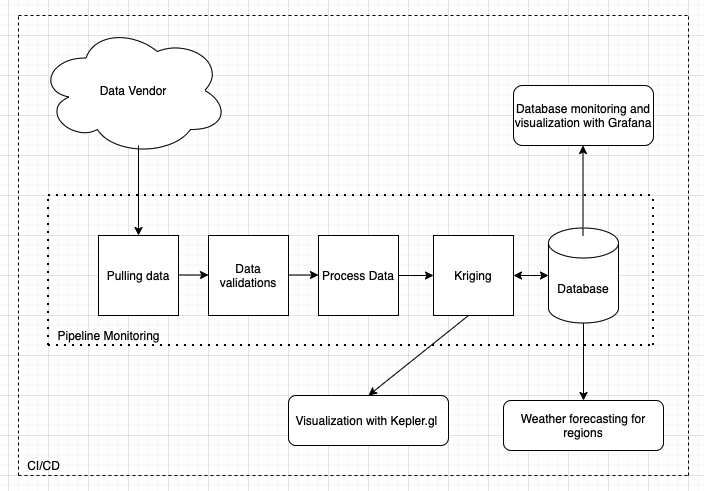
\includegraphics[angle=0,width=0.8\textwidth]{documentation/project_proposal/architecture.png}
\caption{System Architecture}
\end{figure}

\newpage %% prikaz pro pokracovani na nove strance

\section{Technology Specifications}
\noindent 

\subsection{Data}
\noindent There are several key data points that we are interested in for our spatio-temporal dataset.
These include precipitation, humidity, and temperature.
Due to cost constraints, we will have to limit the scope of the data we observe to a smaller region (i.e., Nashville).
However, our system will be designed in such a way that it could be scaled to include larger amounts of data at the cost of the resources required to store and process such data.
Weatherbit.io API provides quality spatio-temporal data available which updates ever 5-25 minutes depending on station reporting frequency. 

\subsection{Data Processing}
\noindent We will use Apache Spark to process the data in the case that it needs to be modified before being moved into the database.
As the Weatherbit.io API only updates every 5-25 minutes, the velocity of the data is low enough for Spark to manage and process the data before moving it into the database.

\subsection{Data Pipeline Monitoring}
\noindent In order to ensure that our system has constant uptime and a high fault tolerance, we will employ a data pipeline monitoring system like Deequ. 

\subsection{Database}
\noindent As our dataset will contain spatio-temporal data, a time-series database is a good choice for our project.
We have chosen to use InfluxDB as it can handle spatio-temporal data and has built in visualization tools and monitoring tools.
As our project is not aimed at created a robust front end client, but rather a pared down data visualization to show the effects of kriging and our forecasting data, this will suit our needs well.
Additionally, InfluxDB is highly performant compared to other potential database options such as Cassandra and will allow our system to be scaled to handle larger geographic regions. 

\subsection{CI/CD}
\noindent In order to maintain constant uptime, we will implement a CI/CD pipeline.
For this purpose, we will use Jenkins as it has widely-available documentation and can be configured with Tugboat on GitHub which will ensure that deployments are successfully built before being launched into production. 

\subsection{Forecasting}
\noindent We will use kriging to fix sparsity in geographical data in order to provide more uniform spatial results in our forecasting.
We will use Pykrige or pyKrigin to accomplish this. 

\subsection{Database Monitoring}
\noindent We will use Grafana to monitor the status and health of our database.
Grafana provides several options for visualizing the state of a database so we will be able to fine-tune the monitoring to our needs and create an alerting system that will inform us of any failures or downtime in the system. 

